\section{Digital design performance}

Quality metrics help to quantify the quality of a design
from different perspectives:

Performance, energy consumption, cost, functionality and robustness.

The most important quality metric is based on application.


\textbf{Performance}

The performance of a digital circuit expresses the computational
load that the circuit can manage.

\textbf{Clock period:} Clock cycle time.

\textbf{Clock rate:} The frequency of the clock.

Circuit performance dpends on the architecture of the processor
(the number of instructions it can execute in parallel)
and the actual design of logic circuitry.


\textbf{Propagation delay}

Propagation delay $t_p$ of a gate defines how quickly it responds
to a change at its inputs.

$$ t_p = \frac{t_{pLH}+t_{pHL}}{2}$$

\begin{center}
	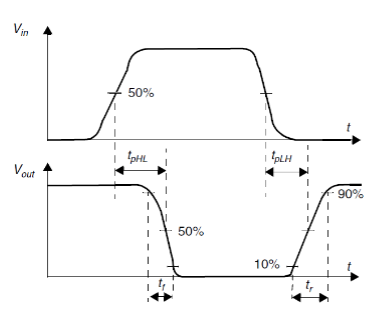
\includegraphics[width=0.5\textwidth]{images/propagationDelay.png}
\end{center}

\textbf{Setup and Hold time}

Setup time is the minimum amount of time before the clock event by
which the input data must be stable for it to be latched correctly.

Hold time is the minimum amount of time after the clock event by
which the input data must be stable for it to be latched correctly.

\begin{center}
	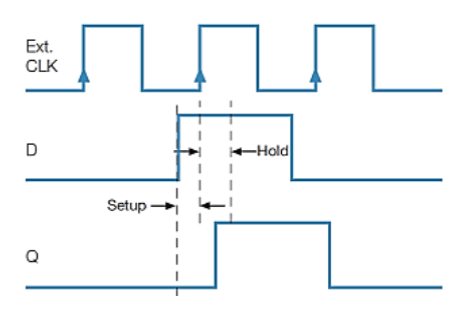
\includegraphics[width=0.5\textwidth]{images/hold.png}
\end{center}

\textbf{Metastable}

A metastable condition occurs when setup or hold times are
violated.

When this happens the digital electronics systems get stuck
for a priod of time.

It's advised to utilize one master clock signal, or several clocks
derived from this master clock. Inputs must be synchronized with
the system clock before being applied to a synchronous system.


\textbf{Clock distribution}

Due to delays associated with routing the clock wires, it may
happen that the clocks become misaligned with respect to each other.
Thus, clock delay or skew.
